%====================================================
%	CHAPTER 4 - Control
%====================================================
\chapter{Controller Development}
\label{ch:control}
%====================================================
\section{Control Loop}
%====================================================
The control problem for this dissertation is, as outlined in Chater:\ref{ch:intro}; to achieve dynamic (\emph{attitude}) set point tracking on a quadrotor by solving the problem of its inherent underactuation. For the purposes of the subsequent controller development, the plant is described in the following non-linear state space form:
\begin{subequations}
\begin{equation}
\dot{\mathbf{x}}=f(\mathbf{x},t)+g(\mathbf{x},\vec{\nu},t)
\end{equation}
\vspace{-15pt}
\begin{equation}
y = c(\mathbf{x},t)+d(\mathbf{x},\vec{\nu},t)
\end{equation}
\end{subequations}
Where the plant dynamics are governed by $f(\mathbf{x},t)$ and the plant's input response by $g(\mathbf{x},\vec{\nu},t)$, for a given input $\vec{\nu}$. The latter is not necessarily a function based relationship and could take a multiplicative form $g(\mathbf{x},t)\vec{\nu}$. The objective for setpoint tracking is that the output to track the state $y = \mathbf{x}$. As such, the control problem is to design a stabilizing control law for an error state $\mathbf{x}_e$:
\\
\vspace{-5pt}
\begin{equation}
\vec{\nu}_d=h(\mathbf{x}_e,t)
\end{equation}
Such that the control plant is globally asymptotically stable or that $\lim_{t\rightarrow\infty}\mathbf{x}_e=0$. It is possible to combine attitude and position states\footnote{Ignoring how error states are formulated for the time being\ldots} into a common trajectory state such that:
\\
\vspace{-5pt}
\begin{equation}
\mathbf{x}=\begin{bmatrix}
\vec{\mathcal{E}}\\
Q_b
\end{bmatrix}
\end{equation}
The body's trajectory is then fully described by $\mathbf{x}(t)$. Independent controllers are developed for attitude and position control and hence attitude and position states aren't combined. However for the purposes of detailing the control plant, a single major loop is considered. The designed control input, $\vec{\nu}_d$, is then implemented by actuator suite $u\in\mathbb{U}$ through its effectiveness function:
\\
\vspace{-5pt}
\begin{equation}
\nu_c=B(\mathbf{x},u,t)
\end{equation}
The exact relationship of the virtual control input and commanded input, $\nu_c\rightarrow\nu_d$, is governed by the allocation algorithm. That allocation function, $B^\dagger$, can be \emph{approximately} referred to as the effectiveness inverse. The actuator positions are then solved subject to some constraint as:
\begin{equation}
u=B^{\dagger}(\mathbf{x},\nu_d,t)
\end{equation}
The control allocation requirements and schemes are expanded upon subsequently in Section:\ref{sec:control.allocation}. Multiple attitude controllers are presented whose stability is proved with Lyupanov$^\dagger$ stability theorem. Each controller is compared in the context of an over actuated quadrotor plant. Similarly a series of allocation schemes are compared too. Those comparisons and their details are presented next in Chapter:\ref{ch:simulation}. 
\newpage
The generalized over-actuated control loop is split into a series of blocks, illustrated in Fig:\ref{fig:control-loop}. From the error state of the generated trajectory, $\mathbf{x}_e$, the control law designs a virtual control input, $\vec{\nu}_d$, which is cast as the argument to the allocation block. From the allocation law, $B^{\dagger}$, physical actuator positions are obtained; $u\in\mathbb{U}$. Those actuator positions effect a virtual plant input, $\vec{\nu}_c$, which progresses the state function. Not shown, but implied in Fig:\ref{fig:control-loop}, is the state derivative feedback of $\dot{\mathbf{x}}$ to the plant transfer function. Finally the output tracking state is estimated with some filtration paradigm, $\hat{\mathbf{x}}=A(\mathbf{x},t)$, and fed back to the error state.
\begin{figure}[htbp]
\centering
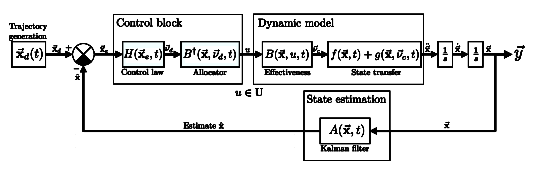
\includegraphics[width=\textwidth]{figs/control-loop}
\caption{Generalized control loop with allocation}
\label{fig:control-loop}
\end{figure}
%====================================================
\section{Control Plant Inputs}
\label{sec:control.inputs}
%====================================================
Thus far control plant inputs for the set of differential state equations, Eq:\ref{eq:quaternion-states}, have mostly been described with net forces and torques; $\mu\vec{F}$ \& $\mu\vec{\tau}$. The relationship between propeller rotational speeds \& servo positions and the resultant thrust vector directions are calculated as in Eq:\ref{eq:quaternion-inputs}.
\begin{subequations}\label{eq:control-input}
\begin{equation}
\mu\vec{F}(u)=\sum Q_{M_i}^*(\lambda_i,\alpha_i)\otimes T(\Omega_i)\otimes Q_{M_i}(\lambda_i,\alpha_i)~~~~\in\mathcal{F}^b
\end{equation}
\vspace{-10pt}
\begin{equation}
\mu\vec{\tau}(u)=\sum \vec{l}\times\big(Q_{M_i}^*(\lambda_i,\alpha_i)\otimes T(\Omega_i)\otimes Q_{M_i}(\lambda_i,\alpha_i)\big)~~~~\in\mathcal{F}^b
\end{equation}
\end{subequations}
To accommodate comparison of each controller and allocation scheme, the error state control law(s) design net plant inputs $\mu\vec{F}$ and $\mu\vec{\tau}$. The allocation rule then takes those net inputs as an arguments to find actuator positions to effect those net inputs. As such each control law can be tested against various allocation rules and \emph{vise versa}. However typical allocation algorithms, like pseudo-inversion, require a multiplicative relationship between plant and control inputs\ldots 
\par
The actuator effectiveness functions in Eq:\ref{eq:control-input} aren't readily able to be reduced to a single multiplicative relationship. Thusly the effectiveness matrix needs an extra layer of abstraction to incorporate a multiplicative relationship. Rather than calculating actuator positions directly from $\vec{\nu}_d$, a set of four 3-dimensional thrust vectors, $\vec{T}_{1\rightarrow 4}$, for each motor module are calculated first.
\begin{equation}
\vec{\nu}_d=\begin{bmatrix}
\mu\vec{F}\\
\mu\vec{\tau}
\end{bmatrix}
= 
\begin{bmatrix}
1 & 1 & 1 & 1\\
\vec{l}_\times & \vec{l}_\times & \vec{l}_\times & \vec{l}_\times
\end{bmatrix}
\begin{bmatrix}
\vec{T}_1\\
\vec{T}_2\\
\vec{T}_3\\
\vec{T}_4
\end{bmatrix}
\end{equation}
Where $\vec{l}_\times$ is the cross product vector of the torque arm. Individual actuator positions for each module, $[\Omega,~\lambda,~\alpha]^T$, can be calculated from those thrust vectors $\vec{T}_i$ for $i\in[1:4]$ with some trigonometry, ensuring that they only adhere to Eq:\ref{eq:control-input}. That trigonometric inversion\footnote{Inverting either rotation matrix operations or quaternions} can be described as the function $R^\dagger$:
\begin{equation}
[\Omega_i,~\lambda_i,~\alpha_i]^T=R^\dagger(\mathbf{x},\vec{F}_i,t)~~~~i\in[1:4]
\end{equation}
\par
Each allocation rule controls designs net thrust vectors for each module in the following form:
\begin{equation}
B^{\dagger}(\mathbf{x},\vec{\nu}_d,t)=\big[ T_{1x},~T_{1y},~T_{1z},~\ldots~T_{4x},~T_{4y},~T_{4z}\big]^T
\end{equation}
The control block in the loop (Fig:\ref{fig:control-loop}) is then modified to incorporate the extra abstraction level, shown in Fig:\ref{fig:control-block}. The output from that control block is still the same actuator matrix $u\in\mathbb{U}$. The block merely accommodates for comparison of various allocation rules without compromising the entire loop's structure.
\begin{figure}[htbp]
\centering
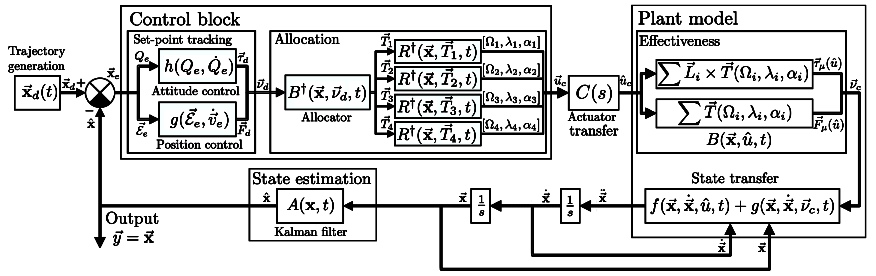
\includegraphics[width=0.7\textwidth]{figs/control-block}
\caption{Abstracted control block}
\label{fig:control-block}
\end{figure}
\par
\emph{\color{Gray} Al allocation algorithms proposed follow the structure described in Fig:\ref{fig:control-block}. One allocation algorithm does, however, circumvent the virtual abstraction level of thrust vector's for each module to directly calculate actuator positions.}
\par
Every control law tested 
\newpage
\subsection*{Model Dependent \& Independent Controllers}
%****************************************************

%****************************************************
\section{Attitude Control}
\label{sec:control.attitude}
%****************************************************
\subsection{The Attitude Control Problem}
\label{subsec:control.attitude.problem}
%****************************************************
\subsection{Quaternion Based Error States}
\label{subsec:control.attitude.quaternion}
%****************************************************
\subsubsection{PD Controller}
%****************************************************
\subsubsection{Auxilliary Plant Controller}
%****************************************************
\subsubsection{PID Controller}
%****************************************************
\subsection{Non-linear Controllers}
\label{subsec:control.attitude.nonlinear}
%****************************************************
\subsubsection{Ideal Back-stepping Controller}
%****************************************************
\subsubsection{Adaptive Back-stepping Controller}
\label{subsubsec:control.attitude.nonlinear.backstep}
\subsubsection*{Disturbance Update Law}
%****************************************************
\subsubsection{Lyupanov Derived Ideal Controller}
%Laselles Theorem
%****************************************************

%****************************************************
\section{Position Control}
\label{sec:control.position}
%****************************************************
\subsection{Backstepping Position Controller}
\label{subsec:control.position.bacstepping}
%****************************************************

%****************************************************
\section{Controller Allocation}
\label{sec:control.allocation}
%****************************************************
\subsection{Pseudo Inverse Allocator}
%****************************************************
\subsection{Weighted Pseudo Inverse Allocator}
%****************************************************
\subsection{Priority Norm Inverse Allocator}
%****************************************************
\subsection{Online Optimized Secondary Goal Allocator}
%****************************************************
\subsection{Non-linear Plant Control Allocation}
\label{subsec:control.allocation.allocators}
%****************************************************